\documentclass[11pt]{beamer}
% \usetheme{Boadilla}
  \usetheme{default}


% acronyms for text or math mode
\newcommand {\ccast} {\mbox{\small CCAST}}
\newcommand {\cris} {\mbox{\small CrIS}}

\newcommand {\airs} {\mbox{\small AIRS}}
\newcommand {\iasi} {\mbox{\small IASI}}
\newcommand {\idps} {\mbox{\small IDPS}}
\newcommand {\nasa} {\mbox{\small NASA}}
\newcommand {\noaa} {\mbox{\small NOAA}}
\newcommand {\nstar} {\mbox{\small STAR}}
\newcommand {\umbc} {\mbox{\small UMBC}}
\newcommand {\uw}   {\mbox{\small UW}}

\newcommand {\fft}  {\mbox{\small FFT}}
\newcommand {\ifft} {\mbox{\small IFFT}}
\newcommand {\fir}  {\mbox{\small FIR}}
\newcommand {\fov}  {\mbox{\small FOV}}
\newcommand {\for}  {\mbox{\small FOR}}
\newcommand {\ict}  {\mbox{\small ICT}}
\newcommand {\ils}  {\mbox{\small ILS}}
\newcommand {\igm}  {\mbox{\small IGM}}
\newcommand {\opd}  {\mbox{\small OPD}}
\newcommand {\rms}  {\mbox{\small RMS}}
\newcommand {\zpd}  {\mbox{\small ZPD}}
\newcommand {\ppm}  {\mbox{\small PPM}}
\newcommand {\srf}  {\mbox{\small SRF}}
\newcommand {\sdr}  {\mbox{\small SDR}}

\newcommand {\ES} {\mbox{\small ES}}
\newcommand {\SP} {\mbox{\small SP}}
\newcommand {\IT} {\mbox{\small IT}}
\newcommand {\SA} {\mbox{\small SA}}

\newcommand {\ET} {\mbox{\small ET}}
\newcommand {\FT} {\mbox{\small FT}}

% abbreviations, mainly for math mode
\newcommand {\real} {\mbox{real}}
\newcommand {\imag} {\mbox{imag}}
\newcommand {\atan} {\mbox{atan}}
\newcommand {\obs}  {\mbox{obs}}
\newcommand {\calc} {\mbox{calc}}
\newcommand {\sinc} {\mbox{sinc}}
\newcommand {\psinc} {\mbox{psinc}}
\newcommand {\std} {\mbox{std}}

% symbols, for math mode only
\newcommand {\wnum} {\mbox{cm$^{-1}$}}
\newcommand {\lmax} {L_{\mbox{\tiny max}}}
\newcommand {\vmax} {V_{\mbox{\tiny max}}}

\newcommand {\tauobs} {\tau_{\mbox{\tiny obs}}}
\newcommand {\taucal} {\tau_{\mbox{\tiny calc}}}
\newcommand {\Vdc}  {V_{\mbox{\tiny DC}}}

\newcommand {\rIT} {r_{\mbox{\tiny\textsc{ict}}}}
\newcommand {\rES} {r_{\mbox{\tiny\textsc{es}}}}
\newcommand {\robs} {r_{\mbox{\tiny obs}}}

\newcommand {\rITobs} {r_{\mbox{\tiny\textsc{ict}}}^{\mbox{\tiny obs}}}
\newcommand {\rITcal} {r_{\mbox{\tiny\textsc{ict}}}^{\mbox{\tiny cal}}}

\newcommand {\ITmean} {\langle\mbox{\small IT}\rangle}
\newcommand {\SPmean} {\langle\mbox{\small SP}\rangle}


\title{Progress Report \\
  Oct--Dec 2014}
\author{L.~L.~Strow \& H.~E.~Motteler}
\institute{
  UMBC Atmospheric Spectroscopy Lab \\
  Joint Center for Earth Systems Technology \\
}
\date{\today}
\begin{document}

%----------- slide --------------------------------------------------%
\begin{frame}[plain]
\titlepage
\end{frame}
%----------- slide --------------------------------------------------%
\begin{frame}
\frametitle{cris tvac}

\begin{itemize}

  \item we show representative results from the {\cris} TVAC tests,
    the PFL side 1 CO, CH$_4$, and CO$_2$ tests, and the MN side 1
    NH$_3$ test

  \item the PFL tests show good agreement with calculated
    transmittances for CO, CH$_4$ and CO$_2$

  \item we also show and representative residuals across the test
    stages

  \item the CO and CH$_4$ side 1 residuals are consistent across the
    MN, PFH, and PFL tests

  \item there was a low-frequency component in residuals in some
    tests

  \item there was a significant difference between nominal and
    observed gas cell pressure in some tests

\end{itemize}

\end{frame}
%----------- slide --------------------------------------------------%
\begin{frame}
\frametitle{test methods}

\begin{itemize}
  \item there is a close parallel between our expression for
    transmittance

    \[\tauobs = f\cdot\SA^{-1}\cdot f \cdot \frac{\FT_2 - \FT_1}{\ET_2 - \ET_1}\]

    and our default \cris\ calibration equation

    \[r_{\mbox{\tiny obs}} = F \cdot r_{\mbox{\tiny ICT}}\cdot f \cdot
    \SA^{-1}\cdot f \cdot \frac{\ES - \SP}{\IT - \SP} \]

  \item here $f$ is a raised-cosine bandpass filter, $\SA^{-1}$ the
    inverse of the ILS matrix, $r_{\mbox{\tiny ICT}}$ is expected ICT
    radiance at the sensor grid, and $F$ is Fourier interpolation
    from sensor to user grid.

  \item the same $f$ is applied to the line-by-line transmittances
    before convolution to the \cris\ sensor grid
 
\end{itemize}

\end{frame}

%----------- slide --------------------------------------------------%
\begin{frame}
\frametitle{CO obs and calc}

\begin{center}
  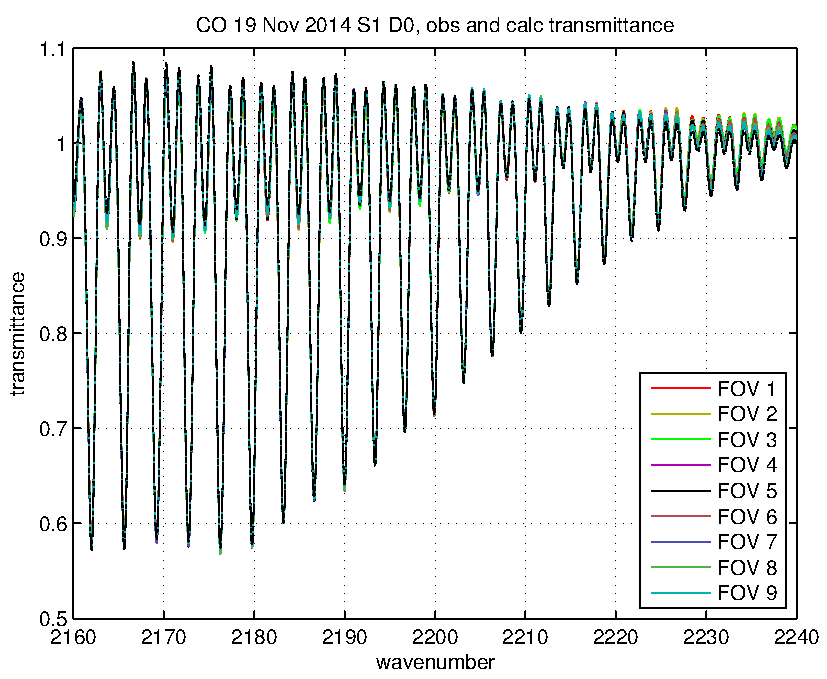
\includegraphics[scale=0.54]{figures/CO_obs_and_calc.pdf}
\end{center}

Observed and calculated transmittance for all FOVs, over the fitting
interval.  At this level of detail we see all values are very close.

\end{frame}
%----------- slide --------------------------------------------------%
\begin{frame}
\frametitle{CO obs minus calc}

\begin{center}
  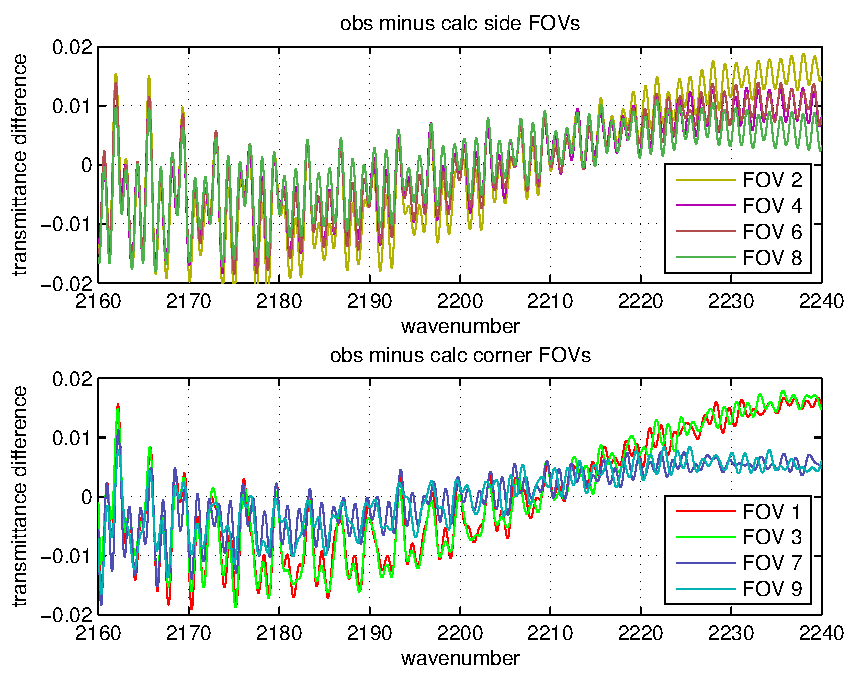
\includegraphics[scale=0.54]{figures/CO_breakout_2.pdf}
\end{center}

Observed minus calculated transmittance for side and corner FOVs,
over the fitting interval.

\end{frame}
%----------- slide --------------------------------------------------%
\begin{frame}
\frametitle{CH$_4$ obs and calc}

\begin{center}
  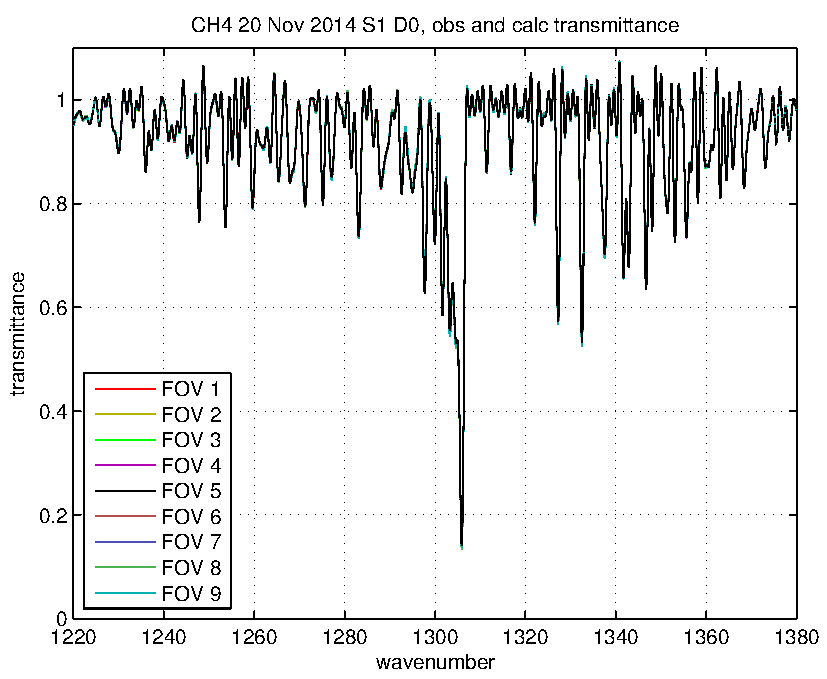
\includegraphics[scale=0.54]{figures/CH4_obs_and_calc.pdf}
\end{center}

Observed and calculated transmittance for all FOVs, over the fitting
interval.  At this level of detail we see all values are very close.

\end{frame}
%----------- slide --------------------------------------------------%
\begin{frame}
\frametitle{CH$_4$ obs minus calc}

\begin{center}
  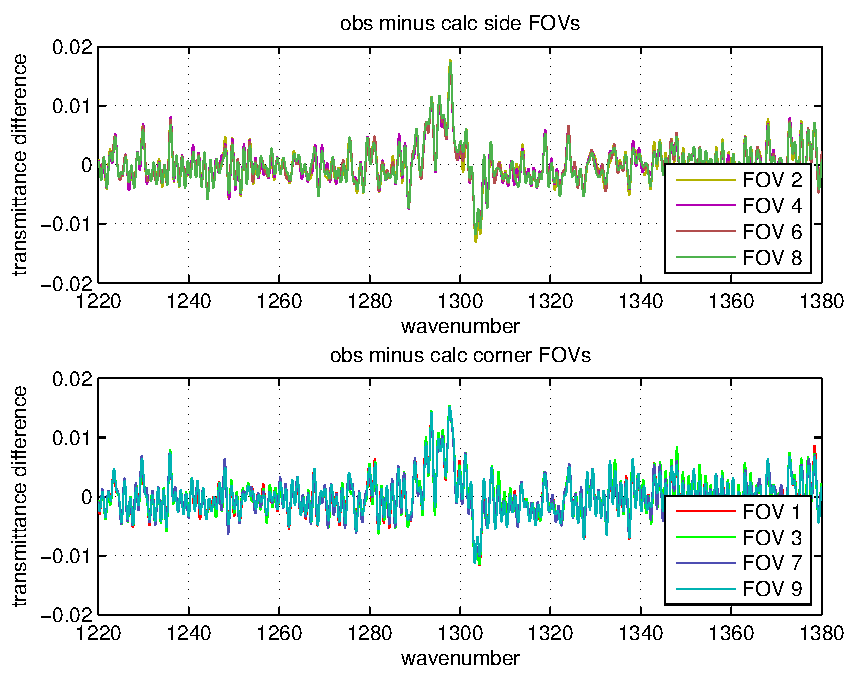
\includegraphics[scale=0.54]{figures/CH4_breakout_2.pdf}
\end{center}

Observed minus calculated transmittance for side and corner FOVs,
over the fitting interval.

\end{frame}
%----------- slide --------------------------------------------------%
\begin{frame}
\frametitle{NH$_3$ obs and calc}

\begin{center}
  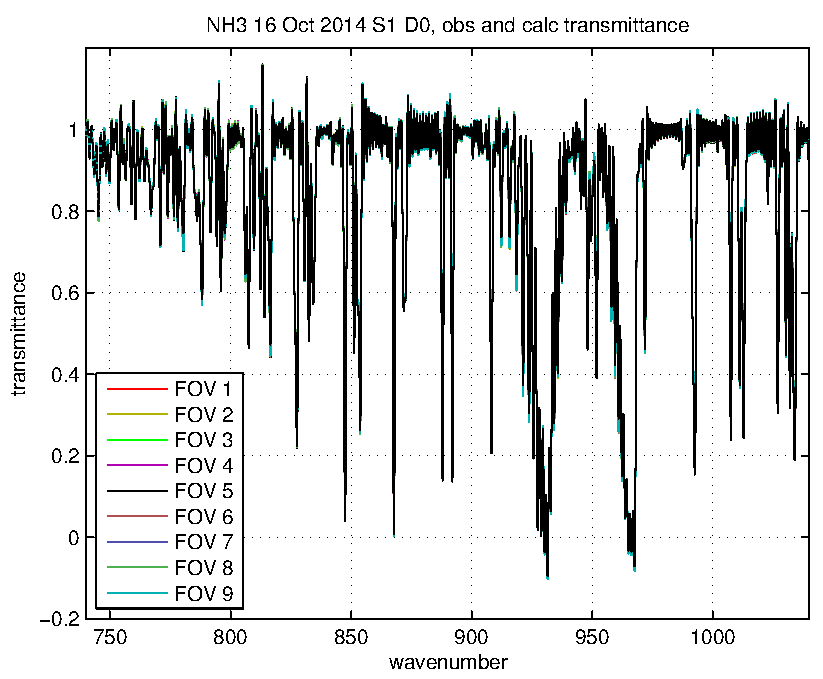
\includegraphics[scale=0.54]{figures/NH3_obs_and_calc.pdf}
\end{center}

Observed and calculated transmittance for all FOVs, over the fitting
interval.  At this level of detail we see all values are close.

\end{frame}
%----------- slide --------------------------------------------------%
\begin{frame}
\frametitle{NH$_3$ obs minus calc}

\begin{center}
  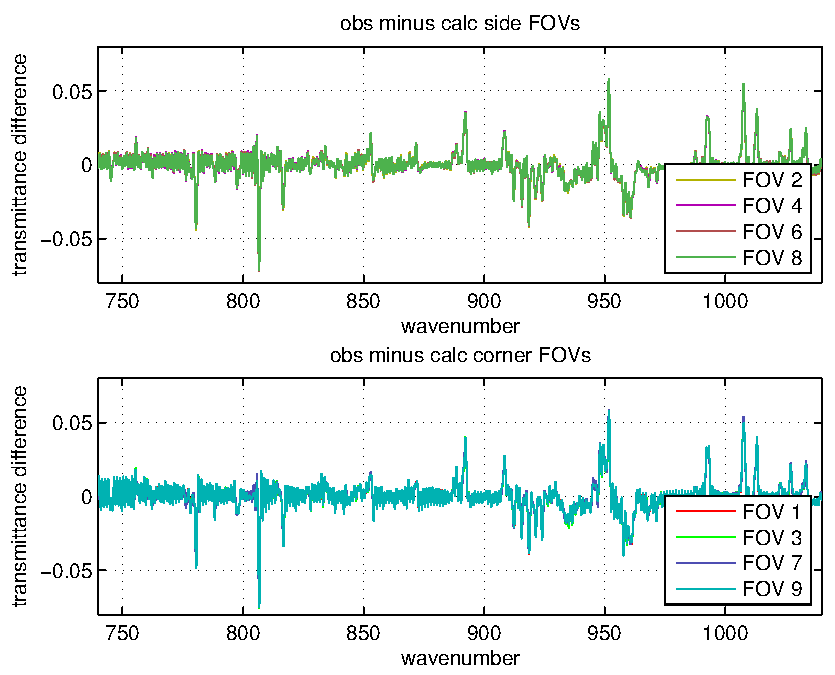
\includegraphics[scale=0.54]{figures/NH3_breakout_2.pdf}
\end{center}

Observed minus calculated transmittance for side and corner FOVs,
over the fitting interval.

\end{frame}
%----------- slide --------------------------------------------------%
\begin{frame}
\frametitle{CO$_2$ obs and calc}

\begin{center}
  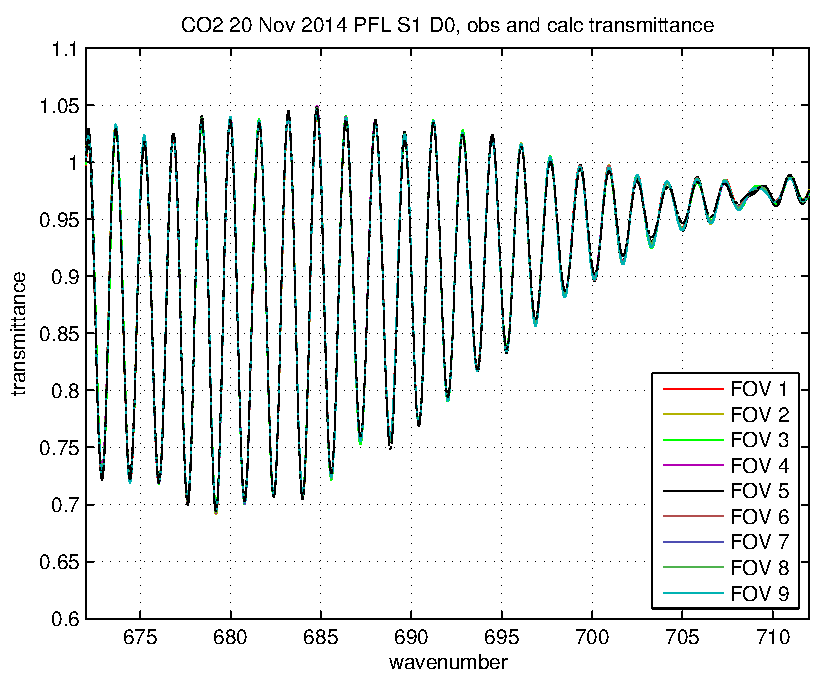
\includegraphics[scale=0.54]{figures/CO2_obs_and_calc.pdf}
\end{center}

Observed and calculated transmittance for all FOVs, over the fitting
interval.  At this level of detail we see all values are close.

\end{frame}
%----------- slide --------------------------------------------------%
\begin{frame}
\frametitle{CO$_2$ obs minus calc}

\begin{center}
  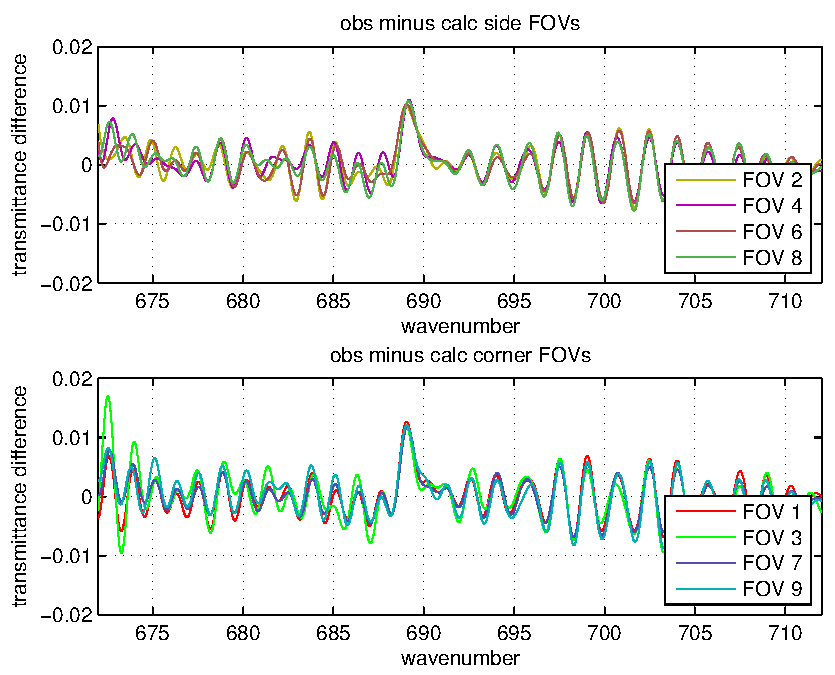
\includegraphics[scale=0.54]{figures/CO2_breakout_2.pdf}
\end{center}

Observed minus calculated transmittance for side and corner FOVs,
over the fitting interval.

\end{frame}
%----------- slide --------------------------------------------------%
\begin{frame}[fragile]
\frametitle{CO side 1 test comparison}

``rms fit'' is $1000 \cdot \rms(a\cdot\tauobs + b - \taucal)$ \\
``met laser'' is the  metrology laser residual

\begin{semiverbatim}\small
          --- rms fit ----        --- met laser --
  FOV    MN      PH      PL      MN      PH      PL  
   1     4.4     1.5     9.9    13.2    15.0    10.3
   2     2.8     3.5    10.6     3.4     5.2     2.3
   3     4.9     2.4    10.0     4.1     2.8     2.6
   4     2.7     3.4     7.7     4.4     6.7     3.9
   5     1.7     2.8     7.9     3.1     3.1     2.6
   6     2.4     3.3     8.1     3.1     2.6     3.6
   7     3.9     1.6     5.3    -0.5    -0.5    -0.8
   8     2.4     3.3     6.5    -6.7    -6.7    -5.7
   9     4.7     2.6     5.2     7.2     4.9     7.5

log torr: MN 40.5 PH 39.9 PL 45.0
obs torr: MN 41.0 PH 26.0 PL 45.0
\end{semiverbatim}

\end{frame}
%----------- slide --------------------------------------------------%
\begin{frame}[fragile]
\frametitle{CO$_2$ side 1 test comparison}

``rms fit'' is $1000 \cdot \rms(a\cdot\tauobs + b - \taucal)$ \\
``met laser'' is the metrology laser residual

\begin{semiverbatim}\small
          --- rms fit ----        --- met laser --
  FOV    MN      PH      PL      MN      PH      PL  
   1     1.6     1.4     3.3     8.3    11.3     0.3
   2     1.6     1.2     3.2     2.1     2.6    -6.2
   3     2.8     1.9     4.0     1.3    -0.3    -4.1
   4     1.8     1.8     3.0     3.6     5.4    -3.1
   5     2.5     2.1     3.4     3.6     4.9    -1.8
   6     2.5     1.6     3.0     2.1     1.8    -3.9
   7     1.7     1.2     3.1    -6.2    -3.9   -13.4
   8     1.8     2.4     3.1    -6.5    -4.9   -11.1
   9     1.7     1.9     3.6     0.8     0.8    -6.2

log torr: MN 40.2 PH 40.0 PL 40.7
obs torr: MN 40.2 PH 40.0 PL 22.0
\end{semiverbatim}

\end{frame}
%----------- slide --------------------------------------------------%
\begin{frame}
\frametitle{notes and comments}

\begin{itemize}
 
  \item we minimize $\rms(a\cdot\tauobs + b - \taucal)$ over 
    the fitting interval as a function of the metrology laser
    wavelength.  From this we get both a conventional residual 
    and the difference of wavelength at the minima from the neon
    calibration value.  The latter value is the ``metrology laser
    residual''

  \item the CO and CH$_4$ side 1 residuals are consistent across the
    MN, PFH, and PFL tests

  \item comparing CO$_2$ tests, the MN and PFH tests were in
    reasonable agreement in comparison with the PFL tests

  \item our NH$_3$ residuals were generally larger than for CO$_2$

  \item all tests shown here were done using UMBC LBL for calculated
    transmittances

  \item to do: derive final focal plane geometery

\end{itemize}

\end{frame}
%----------- slide --------------------------------------------------%
\begin{frame}
\frametitle{ccast high res}

\begin{itemize}

  \item start with \ccast\ and \noaa\ high res data from 6--8 Dec 2014

  \item take the average and standard deviation of \for\ 15 and 16
    independently for each \fov, and compare these values with the
    values for \fov\ 5

  \item results shown here are for 32,186 \ccast\ and 32,120 {\noaa}
    descending {\for}s

  \item as a precaution, {\for}s where any LW channel was greater than
    320K were discarded

  \item the intent is to show variation among {\fov}s, as might arise
    from varying nonlinearity or artifacts of the self-apodization
    correction

\end{itemize}

\end{frame}
%----------- slide --------------------------------------------------%
\begin{frame}
\frametitle{ccast MW mean}

\begin{center}
  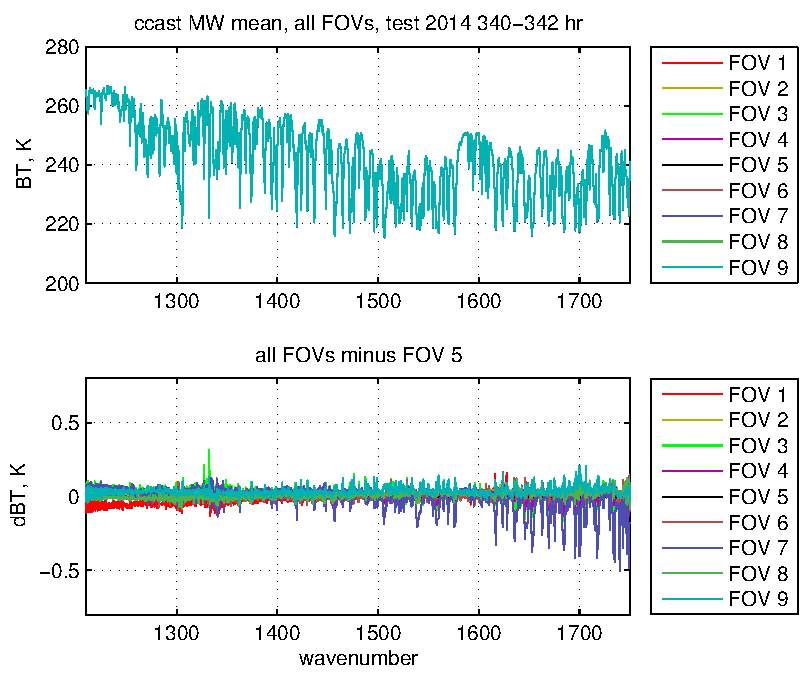
\includegraphics[scale=0.7]{figures/ccast_MW_avg_2014_340-342_hr.pdf}
\end{center}

\end{frame}
%----------- slide --------------------------------------------------%
\begin{frame}
\frametitle{noaa MW mean}

\begin{center}
  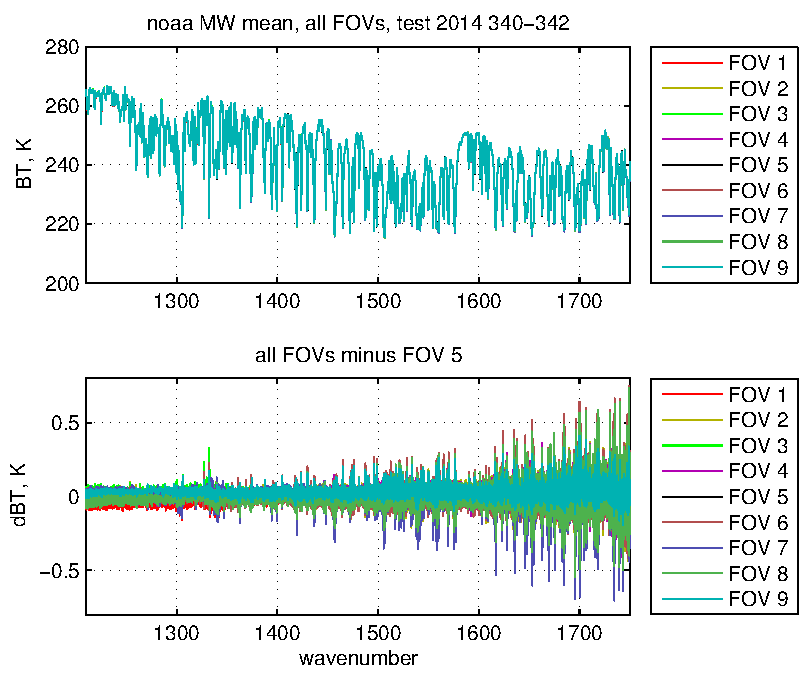
\includegraphics[scale=0.7]{figures/noaa_MW_avg_2014_340-342.pdf}
\end{center}

\end{frame}
%----------- slide --------------------------------------------------%
\begin{frame}
\frametitle{ccast MW fov groups}

\begin{center}
  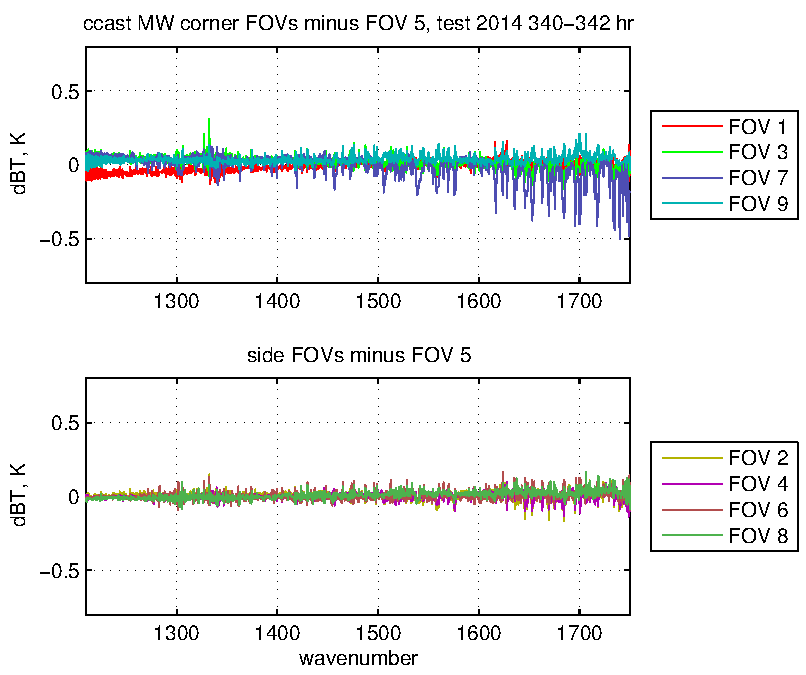
\includegraphics[scale=0.7]{figures/ccast_MW_dif_2014_340-342_hr.pdf}
\end{center}

\end{frame}
%----------- slide --------------------------------------------------%
\begin{frame}
\frametitle{noaa MW fov groups}

\begin{center}
  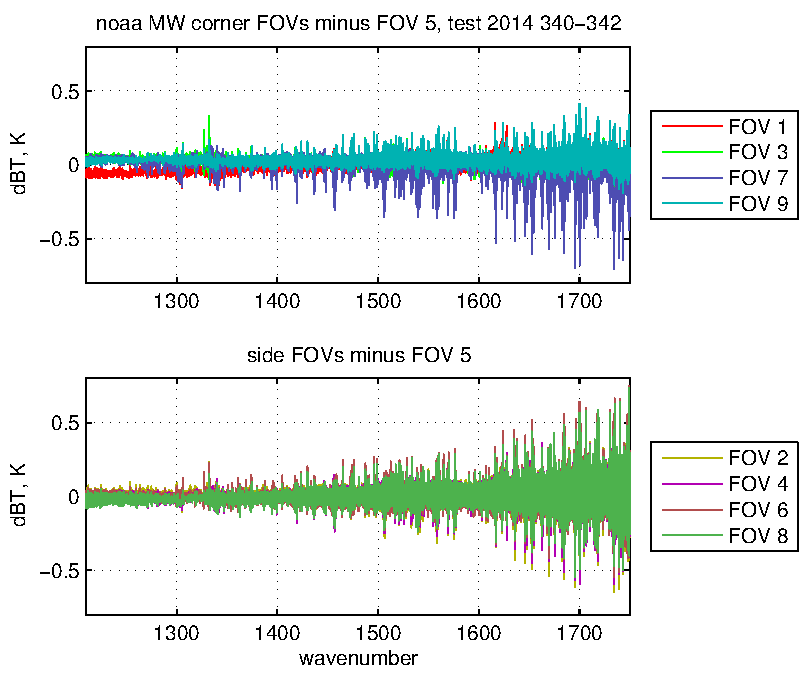
\includegraphics[scale=0.7]{figures/noaa_MW_dif_2014_340-342.pdf}
\end{center}

\end{frame}
%----------- slide --------------------------------------------------%
\begin{frame}
\frametitle{MW discussion}

\begin{itemize}

  \item \fov\ 7 is the least linear, and only partially corrected
    for with the \ccast\ first order adjustment

  \item the \noaa\ variation in \fov\ response is much greater than
    {\ccast}

  \item this may be due to problems with the nonlinearity correction

  \item a normalized frequency domain representation of the numeric
    filter needs a scaling factor to match the original nonlinearity
    measurements.  We used 1.6047 for LW, 0.9826 for MW, and 0.2046
    for SW

\end{itemize}

\end{frame}
%----------- slide --------------------------------------------------%
\begin{frame}
\frametitle{ccast SW mean}

\begin{center}
  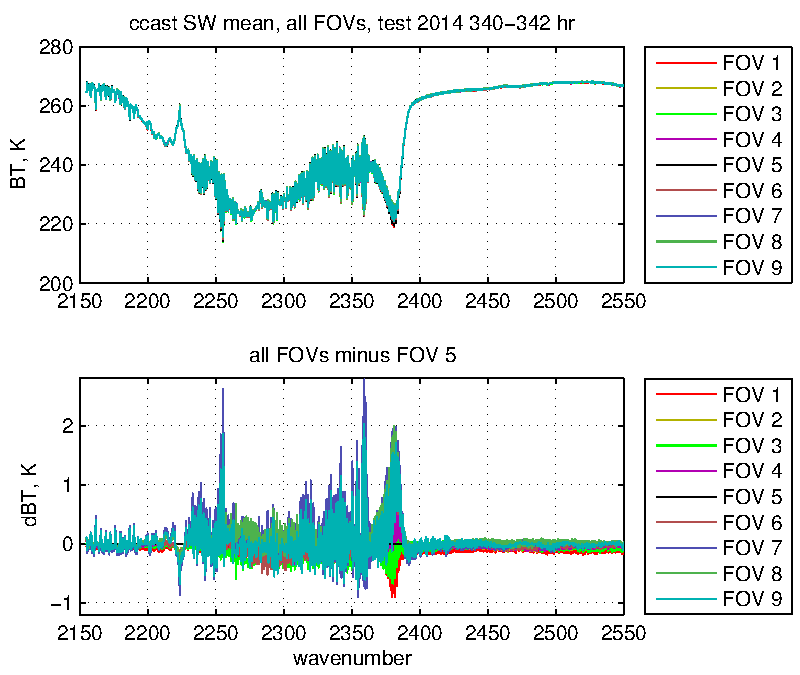
\includegraphics[scale=0.7]{figures/ccast_SW_avg_2014_340-342_hr.pdf}
\end{center}

\end{frame}
%----------- slide --------------------------------------------------%
\begin{frame}
\frametitle{noaa SW mean}

\begin{center}
  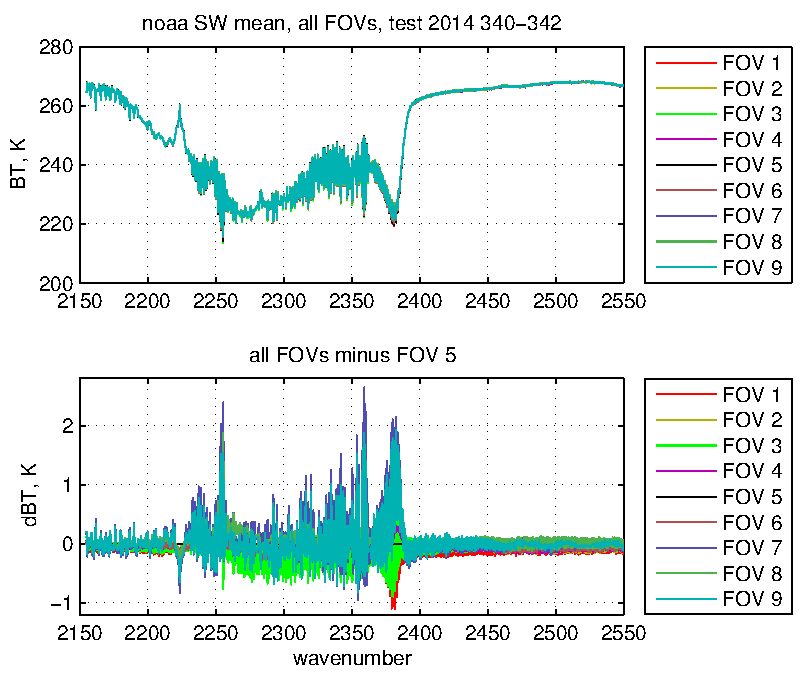
\includegraphics[scale=0.7]{figures/noaa_SW_avg_2014_340-342.pdf}
\end{center}

\end{frame}
%----------- slide --------------------------------------------------%
\begin{frame}
\frametitle{ccast SW fov groups}

\begin{center}
  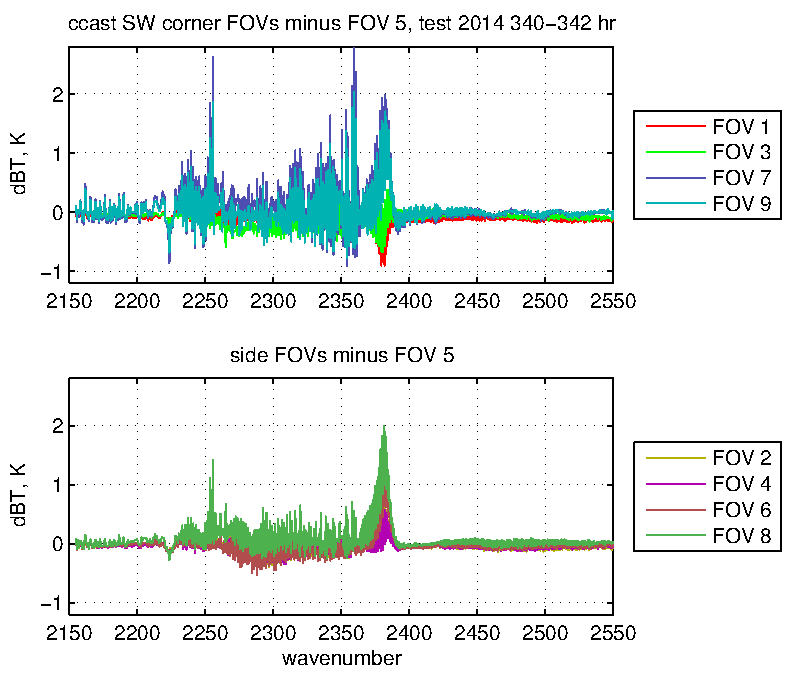
\includegraphics[scale=0.7]{figures/ccast_SW_dif_2014_340-342_hr.pdf}
\end{center}

\end{frame}
%----------- slide --------------------------------------------------%
\begin{frame}
\frametitle{noaa SW fov groups}

\begin{center}
  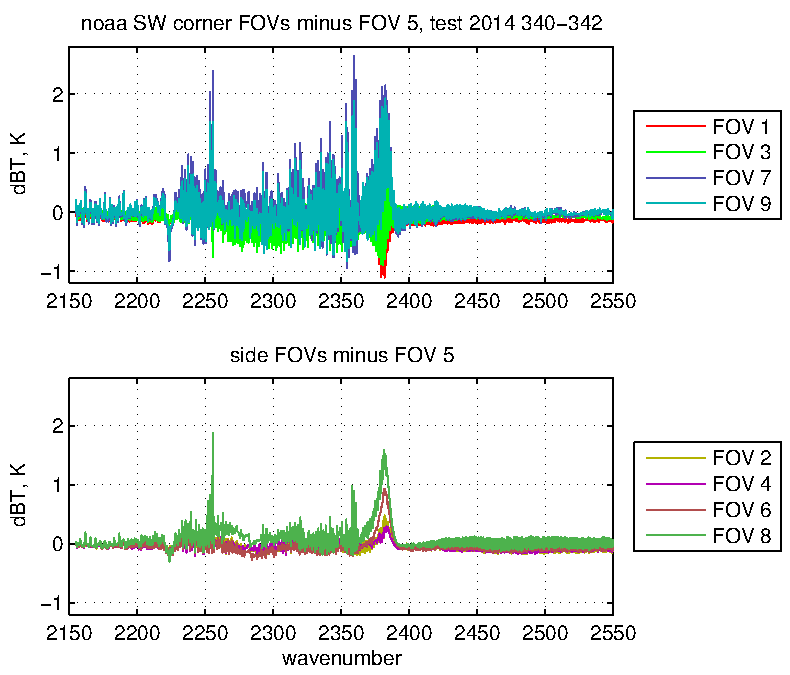
\includegraphics[scale=0.7]{figures/noaa_SW_dif_2014_340-342.pdf}
\end{center}

\end{frame}
%----------- slide --------------------------------------------------%
\begin{frame}
\frametitle{SW discussion}

\begin{itemize}

  \item \ccast\ and \noaa\ are generally in good agreement.

  \item residuals are significantly larger than for the LW band

  \item residuals and \noaa\ vs \ccast\ differences are generally
    greatest for the coldest lines and regions

  \item \fov\ 7 minus \fov\ 5 is significantly greater than for other
    \fov s at 2255 and 2359 \wnum, for both \ccast\ and \noaa

\end{itemize}

\end{frame}
%----------- slide --------------------------------------------------%
\begin{frame}
\frametitle{conclusions}

\begin{itemize}

  \item there is significant convergence in the \ccast\ and
    \noaa\ processing.  We are working with Yong Han's group on the
    MW differences.

  \item variation due to nonlinearity, especially for the MW band, is
    significantly greater than some of the more subtle effects we have
    been considering recently

  \item note again that these results are relative to \fov\ 5 and
    are not comparisons with with expected observed radiance from
    model data or radiance from other sounders

\end{itemize}

\end{frame}
%----------- slide --------------------------------------------------%
\end{document}
